
\begin{figure*}[t]
	\centering
	\begin{subfigure}[t]{.49\textwidth}
		\centering        
		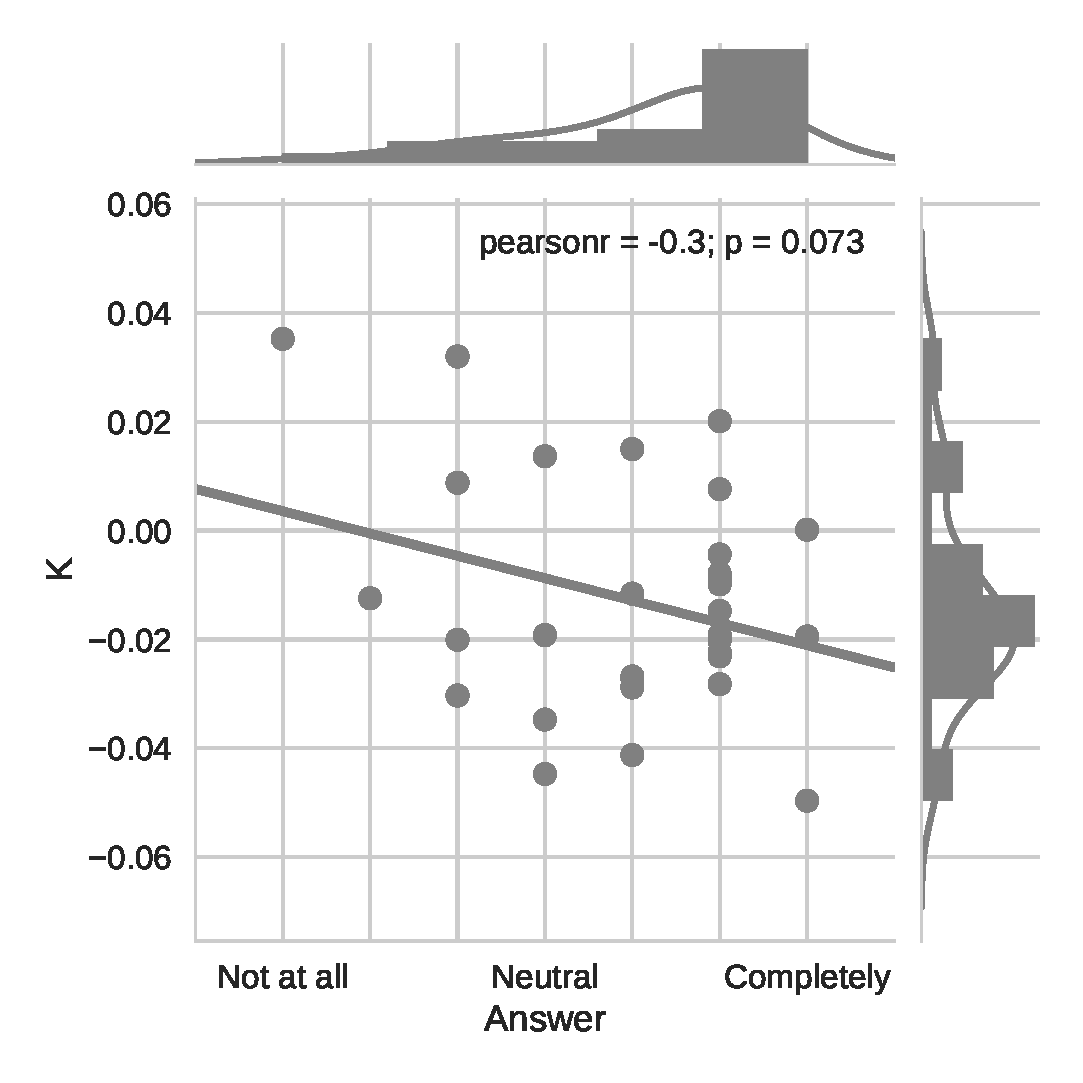
\includegraphics[trim={0cm 0cm 1cm 0cm},clip,width=.8\textwidth]{img/compelling}
		\caption{Correlation between subjective answers to the question \textit{the sense of playing in the remote environment was compelling} in the x-axis and objective metrics values}
		\label{subfig:compelling}
	\end{subfigure}
	\quad
	\begin{subfigure}[t]{.43\textwidth}
		\centering        
		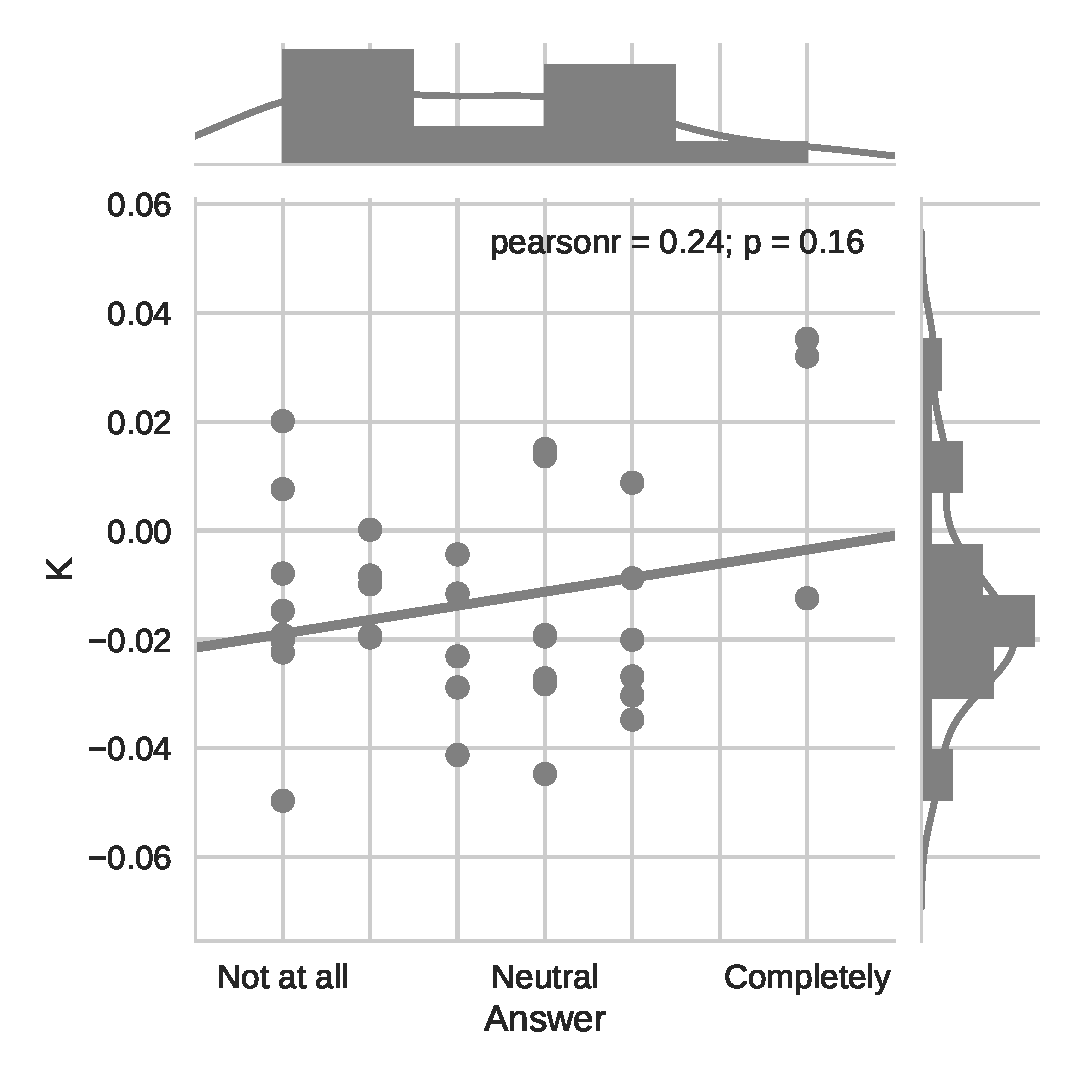
\includegraphics[trim={3cm 0cm 0cm 0cm},clip,width=.8\textwidth]{img/involvement}
		\caption{Correlation between subjective answers to the question \textit{the delay affected the sense of involvement} in the x-axis and objective metrics values}
		\label{subfig:involvement}
	\end{subfigure}
	\quad 
	\caption{Correlation between subjective answers in the x-axis and tempo slope $K$ in the y-axis.}\label{fig:ci}
	%	\vspace{-1em}
\end{figure*}  


\section{Results and discussion}\label{sec:discussion}
Though limited in the amount of involved people and performances, the experiments described in the previous section were helpful to start the discussion about the pedagogical applications of NMPs with musicians, and to collect useful comments and suggestions that will guide our investigation. 


\subsection{Objective, subjective and biological metrics}\label{subsec:metrics}
In the two experiments, we investigate the sense of presence and quality of performance of the couple of subjects in case of visual occlusion (co-presence experiment) and different network latency conditions (networked performance). The acquisition and evaluation was performed using subjective and objective metrics \cite{CIM2018}. 

With regard to the former, we used a post-experiment 27-item questionnaire divided in five main topics, such as \textit{Predictability and Interaction}, or \textit{Quality of the Music Performance}. After each phase of the networked experiments, we asked a subset of five questions to evaluate the impact of different latency conditions in the questionnaire.

With regard to the latter, we acquired the audio recordings of the networked performance, manually tracked the beat, extracted a BPM trend and computed a degree of acceleration/deceleration $K$  (\textit{tempo slope}) from it. Other metrics used in NMP literature include the pacing, the regularity or the imprecision of the performance \cite{RottondiOverview}.

It is interesting to observe the comparison between the subjectively-perceived quality of the performance and the  objective metrics computed from the corresponding audio recording. In Figure \ref{fig:ci} we show the comparison with the answers to two quality-related questions, i.e., \textit{the sense of playing in the remote environment was compelling} (Fig. \ref{subfig:compelling}) and \textit{the delay affected the sense of involvement} (Fig. \ref{subfig:involvement}).

Due to the few samples we obtained, it is not possible to draw statistically-meaningful conclusions. The preliminary observations, however, show an interesting trend that we would like to investigate further. The musicians seem to be more compelled with the remote environment when the levels of $K$ were lower, i.e., when the tendency to slow down is more accentuated. Analogously, their sense of involvement in the performance show little correlation with the tempo trend. 

Two musicians, indeed, can easily keep the tempo by making one subject following the lead of the other, using a master-slave approach to cope with latency \cite{Carot07networkmusic}. In this case musicians would not improve their musical skills to interact with partners. From these results, we can infer that $K$ is not suitable to be used as an objective metrics of the subjective satisfaction of subjects. 

A first investigation in the project will be devoted to find a content-based metrics that is coherent with the pedagogical purposes of NMPs and suitable for providing a 
%We aim to extract such a metrics using content-based techniques, in order to provide a 
useful feedback for students.% and can guide our research for a more effective platform for NMP. 
This study will involve acquiring %to We may estimate metrics from the level of comfortability of the students during a lesson or a rehearsal. For this reason, we intend to acquire 
biometric signals to estimate the level of distress during the performance and to investigate whether the NMPs contribute to increase such level. 

\subsection{Auditory and visual feedback}
After the experiments, we asked musicians about the strategies they adopt for 
%From the co-presence experiment, we could observe different strategies of 
musical coordination and interpretation, which they report to be based on breathing signaling and communicative gestures to keep synchronization, especially for attacks and the duration of sustained notes. In the co-presence experiment, %is case, 
the no-sight condition deeply affected the expressiveness of the performance. In full visual occlusion, the performers relied mostly on acoustic cues to keep the tempo, with the apparent effect of an acceleration during the performance. 

\begin{figure}[b]
	\centering
	\begin{subfigure}[t]{.48\columnwidth}
		\centering        
		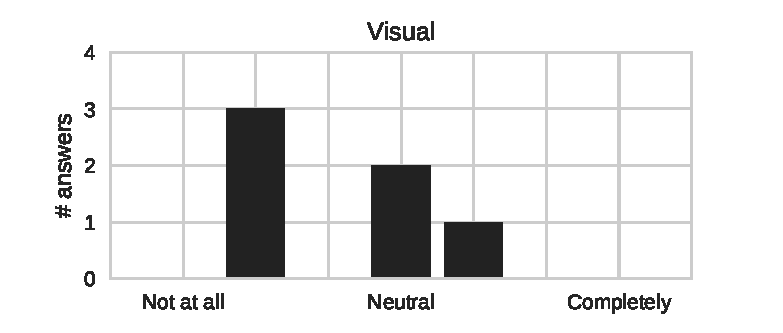
\includegraphics[trim={.5cm 0cm 1cm 0cm},clip,width=\textwidth]{img/Visual}
		\caption{Influence of the visual feedback}
		\label{subfig:visual}
	\end{subfigure}
	\begin{subfigure}[t]{.48\columnwidth}
		\centering        
		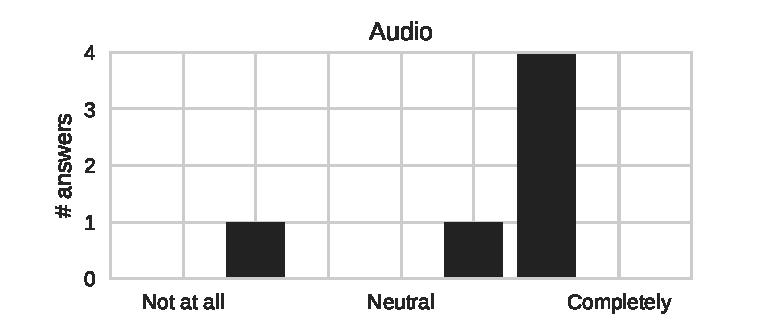
\includegraphics[trim={1.5cm 0cm 0cm 0cm},clip,width=\textwidth]{img/Audio}
		\caption{Influence of the auditory feedback}
		\label{subfig:audio}
	\end{subfigure}
	\quad 
	\caption{Histogram of the answers on the influence of visual and auditory feedback after the NMP experiment.}\label{fig:va}
	%	\vspace{-1em}
\end{figure}  

This aspect is also investigated in the remote performance by asking in the perceptual questionnaire how much the visual and auditory display quality interfered or distracted them from performing. In Figure \ref{fig:va} we display a histogram of the answers in a 7-point likert scale. While the influence of the visual feedback is limited (Fig \ref{subfig:visual}), the auditory feedback is predominant for the performance.

During the time of free comments, the subjects explained that the video feedback was less relevant due to the low degree of synchronicity introduced by the latency, which led them to look less for a visual interaction with their partner. In order to translate these comments into requirements for a NMP tool, we need to assess the importance of visual and auditory interaction in performances and rehearsal. A level of auditory interaction can be estimated using a measure of asymmetry between the audio recordings of the two subjects, as computed in \cite{Chafe3}. With regard to visual interaction, we intend to acquire a video recording of the performance using cameras that capture when the subjects are watching at their partners on the screen. By annotating both intentional and saccadic movements, we aim at estimating whether a higher level of interaction between subjects corresponds to higher satisfaction in the performance and, possibly, how to design the visual and auditory feedback in our platform.
 
\subsection{Peripheral visual feedback}
In the previous subsection, we discussed the importance of visual feedback in co-presence and networked performances. During the co-presence experiment, we observed how performers where comfortable with blurred visual of their partners. They referred us that most of the information for synchronization is contained in the perception of motion from the partners, rather than in the full view.

In the networked experiment the subjects were placed in front of webcam and monitor in order to improve eye contact, as in \cite{duffy2017new}. Some participants of the networked performances commented that one of the reason of the influence of the visual feedback was the lower importance of direct visual interaction. In their typical disposition during rehearsal and performance they are placed in front of an audience rather than in front of each other and, therefore, mostly rely on peripheral vision for interacting.

As next steps, we intend to test the role of peripheral vision by trying different arrangement of video equipment and subjects during the NMPs. This involves to test different virtual environments and find the most promising for pedagogical purposes.  The most suitable arrangements may involve use multiple visual feedbacks, e.g., one frontal for eye contact and one for catching peripheral motion. This would mean dealing with multiple video streams, which demands a larger bandwidth. Reducing the demand in terms of bandwidth is nonetheless desirable in order to improve the spread of our tools. We intend to investigate on strategies to decrease the need of bandwidth.


\begin{figure}[t]
	\centering
	\begin{subfigure}[t]{.46\columnwidth}
		\centering        
		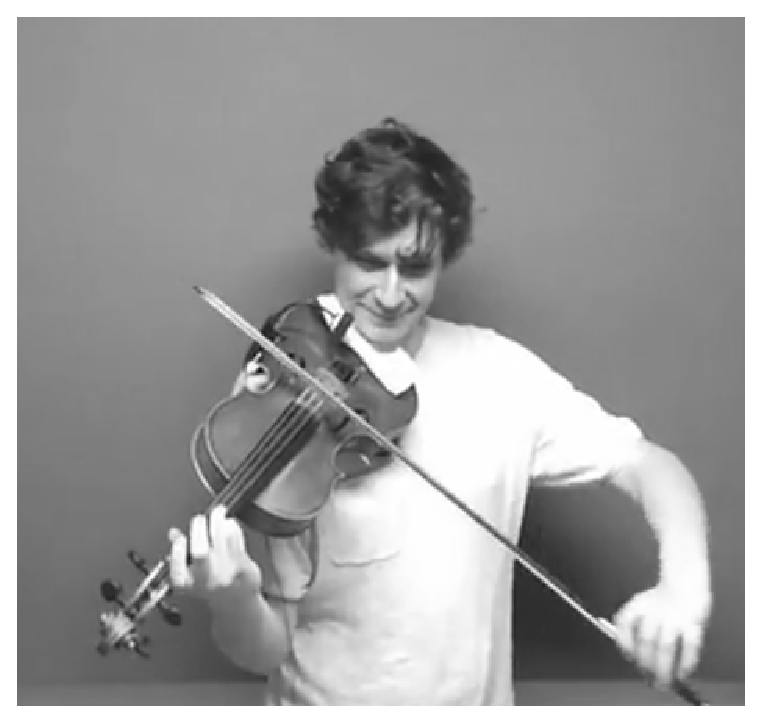
\includegraphics[trim={0cm 0cm 0cm 0cm},clip,width=\textwidth]{img/webcam}
		\caption{Normal view}
		\label{subfig:webcam}
	\end{subfigure}
	\quad
	\begin{subfigure}[t]{.46\columnwidth}
		\centering        
		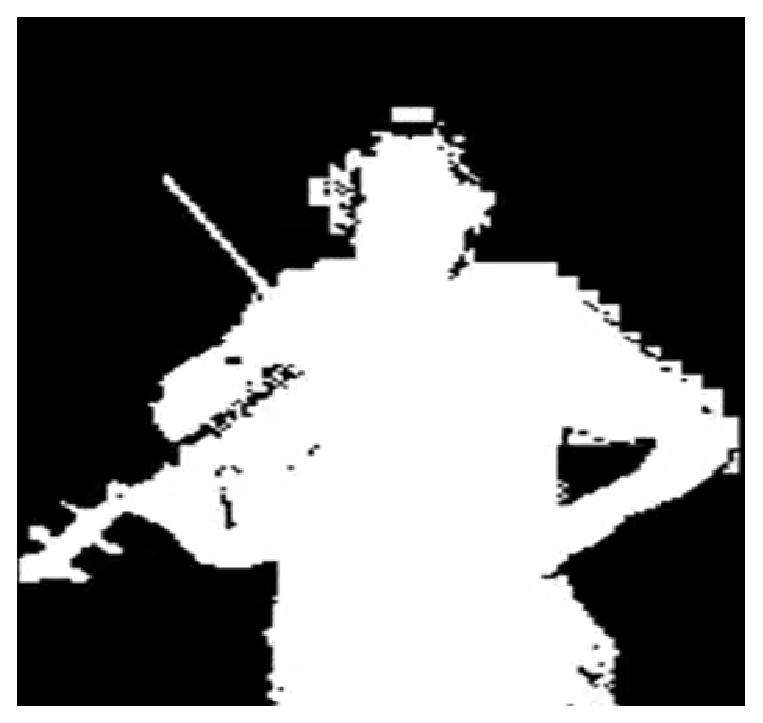
\includegraphics[trim={0cm 0cm 0cm 0cm},clip,width=\textwidth]{img/blob}
		\caption{BLOB view}
		\label{subfig:blob}
	\end{subfigure}
	\quad 
	\caption{Comparison between normal and BLOB view of a musician during a NMP.}\label{fig:wb}
	%	\vspace{-1em}
\end{figure}  


Both LOLA and Ultragrid implement several coding algorithm to reduce the bandwidth, while slightly increasing the processing time for coding/decoding the video streams \cite{drioli2013networked,holub2006high}. A higher saving would be to detect and transmits only the silhouette of the musicians as a binary large object (BLOB) \cite{camurri2010visual}. In Figure \ref{fig:wb} we show a comparison between a normal take of a musician (Fig. \ref{subfig:webcam}) and a BLOB view (Fig. \ref{subfig:blob}).
Being a binary image, the BLOB view is extremely lighter, while keeping most of the information on the motion. As future directions, we intend to investigate whether the BLOB or other motion-related representations can effectively convey the information needed by musicians for rehearsing together. 


\subsection{Mono vs Stereo vs 3D Audio}
Monophonic audio acquisition and rendering is commonly used in NMPs \cite{CIM2018}. Some studies employ headphones to avoid audio loops \cite{RottondiFeature}, while others use monophonic speakers and echo-cancellation algorithms for avoiding feedbacks \cite{drioli2013networked}. 

The directionality of the sound is crucial %can be neglected for duo rehearsal or teacher-student lessons, but it is important 
in case of performances with many musicians, where it helps locating the sources and improving the ability to focus on the instruments separately. 

We intend to investigate the influence of sound directionality in NMPs by testing different audio conditions and verifying which one the musicians prefer. A first condition is to use panning with headphones and stereo speakers to place the sound sources. A second condition is to use binaural rendering for headphones and more accurate methods for the stereophonic location of the sounds. Lastly, we want to use an array of speakers in different arrangement to allow more accurate rendering of sound fields. 

It is also worth mentioning that it is not natural for musicians to wearing headphones during a performance, as they also affect their ability to hear their own sound. Moreover, to properly locate the sound sources in the virtual environment, the binaural rendering requires a proper head tracking algorithm to constantly update the location of sources with respect to the orientation of the listener \cite{Bonacina2016}.

There are further scenarios where a 3D acquisition of the sound field is required.  Most instruments have indeed a clear pattern of radiance and listening to them from different angles lead to sensible changes of the timbral properties \cite{CancliniAES}. In a teacher-student scenario, a teacher may be interested to have a richer information to assess the progress of their students. We aim to employ state-of-the-art techniques for the plenacoustic analysis and rendering, as in \cite{Canclini2015}.

%Even in case of a student-teacher lesson, a more directional acquisition may be required. Most instruments have indeed a clear pattern of radiance and listening to them from different angles lead to sensible changes of the timbral properties \cite{CancliniAES}. In this situation, a teacher may be interested to have a richer information to assess the progress of their students. We aim to employ state-of-the-art techniques for the plenacoustic analysis and rendering, as in \cite{Canclini2015}.

\subsection{Matching acoustics of environments}
In the networked experiment we did not take the influence of room acoustics for the performance into consideration. In other experiments, the performers play in acoustically insulated and semi-anechoic rooms to remove this influence \cite{RottondiFeature}. Musicians have difficulty playing in semi-anechoic rooms, as the perceived timbre of instruments change dramatically making hard for them to recognize the quality of their performance \cite{Woszczyk2009}.

In real-case scenarios, it is likely that musicians are going to perform over network from two acoustically-different environments. In this case, they would listen to their own sound colored by their environment and receive their partner audio signal from a different acoustic, creating a misalignment between the two environments.

In future work, we want to take the effect of environment acoustic into account by testing different combinations of real rooms' acoustics and synthetically-processed acoustics~\cite{Boucher15}. This will help us understanding if musicians require techniques to address the issue of different acoustic environments for having a realistic performance. These techniques may involve to first blindly assess the acoustic conditions of the two environments and then de-convolve the partner's audio stream \cite{CancliniRoom}.



\subsection{Measure for latency compensation and virtual conductor}
One of the main factor investigated in the NMP literature was the influence of network latency in the quality \cite{RottondiOverview,drioli2013networked}, as we also did in the networked experiment. The new 5G network is showing promising results for enabling low-latency connections, that may enable NMPs applications even for generic users \cite{uk5G}. Nevertheless, a certain amount of latency is likely to be present for NMPs using general purpose hardware and connections. 

For this reason, researchers have been developing strategies to cope with the latency. In \cite{Carot07networkmusic} the authors identify a set of strategies such as the laid-back approach, which involves for a musician to play slightly behind the beat, and the delayed feedback approach, which involves to equip one of the musician with a delayed feedback of their own sound in order to synchronize it with their partners sound. The presence of a conductor has also been shown to increase the tolerance to delay, thanks to the shared cue provided to the performers \cite{Olmos2009}.

In the project, we aim to develop algorithms that help musicians compensating for the delay. We plan to use a beat tracker to dynamically track the rhythm of the performance of the musicians, as in \cite{Goto2010}, and provide it in advance to musicians. This will allow musicians to follow a virtual conductor, similarly to what proposed in \cite{conductor2008}.
